\begin{figure}[htbp]
\section*{ CTCF}
\centering
\begin{subfigure}[b]{0.95\textwidth}
\centering
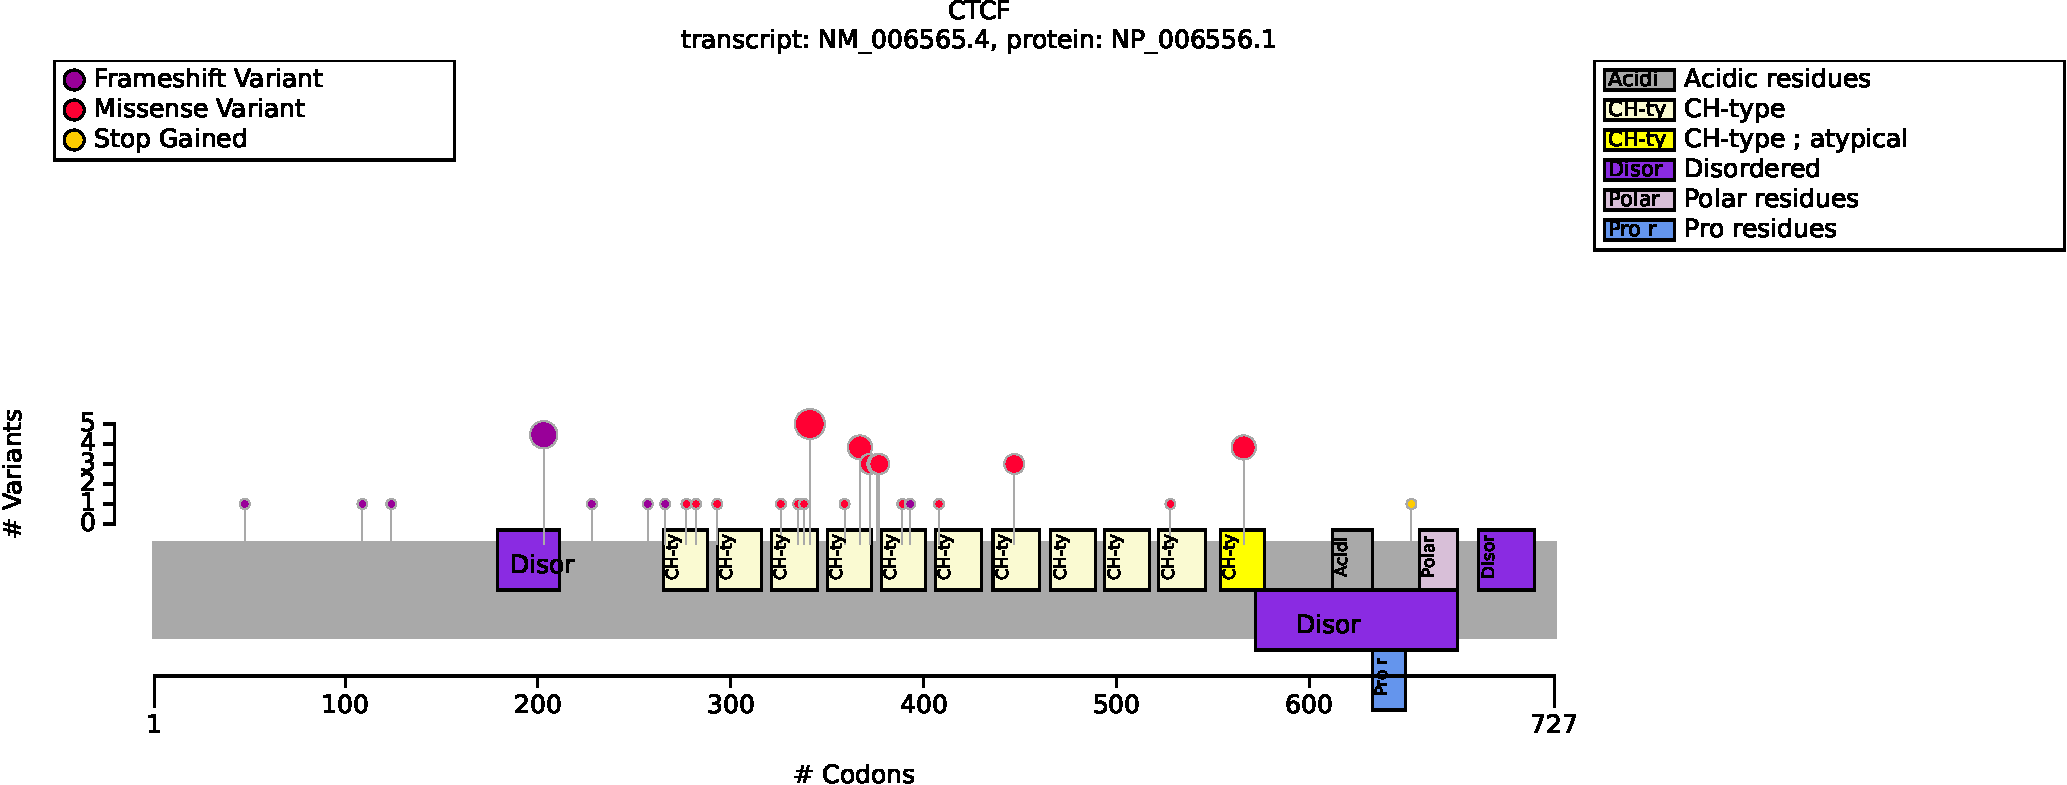
\includegraphics[width=\textwidth]{ img/CTCF_protein_diagram.pdf} 
\captionsetup{justification=raggedright,singlelinecheck=false}
\caption{Distribution of variants in CTCF}
\end{subfigure}

\vspace{2em}

\begin{subfigure}[b]{0.95\textwidth}
\centering
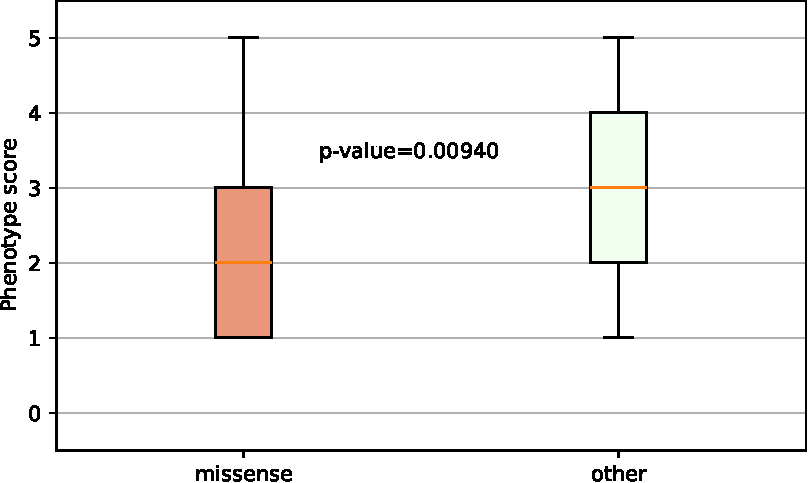
\includegraphics[width=0.3\textwidth]{ img/CTCF_stats.pdf} 
\captionsetup{justification=raggedright,singlelinecheck=false}
\caption{DeVries score to compare CTCF missense vs other variants.}
\end{subfigure}

\vspace{2em}

\begin{subfigure}[b]{0.95\textwidth}
\centering
\resizebox{\textwidth}{!}{
\begin{tabular}{llllrr}
\toprule
Genotype (A) & Genotype (B) & total tests performed & significant results\\
\midrule
missense & other & 27 & 0\\
\bottomrule
\end{tabular}
}
\captionsetup{justification=raggedright,singlelinecheck=false}
\caption{Fisher Exact Test performed to compare HPO annotation frequency with respect to genotypes.}
\end{subfigure}

\vspace{2em}

\begin{subfigure}[b]{0.95\textwidth}
\captionsetup{justification=raggedright,singlelinecheck=false}
\resizebox{\textwidth}{!}{
\begin{tabular}{llllrr}
\toprule
Description & Variable & Genotype (A) & Genotype (B) & p-value & xrefs\\
\midrule
A phenotypic severity score for individuals with intellectual disability & De Vries score & missense & other & 0.009 & -\\
\bottomrule
\end{tabular}
}
\caption{ De Vries Score to compare missense and other with respect to De Vries score. }
\end{subfigure}

\vspace{2em}

\caption{The cohort comprised 46 individuals (18 females, 28 males). A total of 110 HPO terms were used to annotate the cohort. 
Disease diagnosis: Intellectual developmental disorder, autosomal dominant 21 (OMIM:615502). Previously, a group
did not observe a correlation between the location of the variants and the overall severity of various phenotypes, 
including the level of intellectual function, presence of congenital anomalies, or poor growth \cite{PMID_36454652},
but analysis using a score such as the DeVries score was not attempted.
A total of 46 unique variant alleles were found in \textit{CTCF} (transcript: \texttt{NM\_006565.4}, protein id: \texttt{NP\_006556.1}).}
\end{figure}
